\documentclass[11pt]{article}

% Change "review" to "final" to generate the final (camera-ready) version.
\usepackage[review]{acl}

% Standard package includes recommended by the ACL template
\usepackage{times}
\usepackage{latexsym}
\usepackage[T1]{fontenc}
\usepackage[utf8]{inputenc}
\usepackage{microtype}
\usepackage{inconsolata}

% Additional packages you were using
\usepackage{amsmath, amssymb}
\usepackage{graphicx}
\usepackage{hyperref}
\usepackage{cleveref}
\usepackage{enumitem} % for list control
% Add these packages to the preamble (near your other \usepackage lines)
\usepackage{pgfplots}
\pgfplotsset{compat=1.17}
\usepackage{caption}
\usepackage{subcaption} % optional, if you want subfigures later
% If title/author block needs more space, uncomment and change:
% \setlength\titlebox{6cm}
\usepackage{float}
\usepackage{xcolor}
% \YRMcommentstrue makes \YRM show comments, \YRMcommentsfalse makes it do nothing.
\newif\ifYRMcomments
\newif\ifBacklogcomments
\newif\ifResolvedcomments

\YRMcommentstrue % set to \YRMcommentsfalse to hide comments
% \YRMcommentsfalse
\Backlogcommentstrue
% \YRMBacklogcommentsfalse
\Resolvedcommentstrue


\newcommand{\YRM}[1]{\ifYRMcomments\textcolor{red}{[YRM: #1]}\fi}

\newcommand{\Backlog}[1]{\ifBacklogcomments\textcolor{blue}{[Backlog: #1]}\fi}

\newcommand{\Resolved}[1]{\ifResolvedcomments\textcolor{green}{[Resolved: #1]}\fi}


\title{Attention Sink Mechanisms Are Not Universal Across Different Transformer Architectures}

\author{First Author \\
  Affiliation / Address line 1 \\
  Affiliation / Address line 2 \\
  \texttt{email@domain} \\\And
  Second Author \\
  Affiliation / Address line 1 \\
  Affiliation / Address line 2 \\
  \texttt{email@domain} \\
}

\date{}

\begin{document}
\maketitle

\begin{abstract}
  Transformers commonly exhibit an attention sink: disproportionately high attention to the first position. We study this behavior in GPT-2–style models with learned query biases and absolute positional embeddings. Combining analysis with targeted interventions, we find that the sink arises from the interaction among (i) a learned query bias, (ii) the first-layer transformation of the positional encoding and (iii) structure in the key projection. Together with observations of sinks in models without query biases or absolute positional embeddings (e.g., RoPE or ALiBi), this indicates that attention sinks do not arise from a single universal mechanism but instead depend on architecture. These findings inform mitigation of attention sink, and motivate broader investigation of sink mechanisms across architectures and training regimes.
\end{abstract}

\section{Introduction}


\section{Related Work}
\YRM{I didn't look at this part yet, waiting for you to finish it fist :) } 

\YRM{As mentioned, this needs to be improved - By citing more, making this more concise (as concise as possible while including really vital info, and adding more in appendix if needed, like we did in our attention knockout paper )}Our investigation into the attention sink's origins builds upon four key areas of Transformer research: the methods for encoding positional information, the phenomenon of attention sink, and the recent discovery of massive activations functioning as implicit biases.

\subsection{Positional Encoding in Transformers}
By design, the self-attention mechanism has no inherent sense of token order. To address this, Transformers must be augmented with positional information. The original Transformer used fixed sinusoidal embeddings \cite{vaswani2017attention}. Many models in the GPT family, including the GPT-2 model we investigate, use learned absolute positional embeddings - a vector for each position that is added to the token embedding at input. More recent architectures have introduced alternative methods, such as the LLaMA architecture \cite{touvron2023llama2} which utilizes Rotary Positional Embeddings (RoPE) \cite{su2021roformer}, and Attention with Linear Biases (ALiBi) \cite{press2021train}, which is a key feature in models like BLOOM \cite{bigscience2023bloom}.

\subsection{The Attention Sink Phenomenon}
Recent empirical work has identified a curious and robust phenomenon in auto-regressive language models termed the ``attention sink'' \cite{xiao2023efficient}. This refers to the tendency of models to allocate a significant portion of their attention to the very first token(s) in a sequence, even when these tokens are not semantically important. As \cite{gu2025when} demonstrate, this phenomenon is not an anomaly but emerges consistently during pre-training. Some studies have found the attention sink could have a negative impact on the achievable accuracy of LLMs \cite{Yu2024Unveiling}. Some models, such as Mamba-based models as \citet{endy-etal-2025-mamba} shows, don't exhibit attention sink. \Resolved{When working on this part, please make sure to cite my paper (attention knockout), it related to this paper because there we show that Mamba-based models don't have an attention sink so we can cite it as papers showing that some architecture don't suffer from attention sink (it's common practice  to forcibly cite yourself haha)}

\subsection{Massive Activations}
The phenomenon of \emph{massive activations}—where a tiny subset of coordinates exhibit orders-of-magnitude larger activations—has been identified and characterized across a variety of LLMs (\cite{sun2024massive}, \cite{lindnielsen2024spectral}, \cite{lin2024duquant}). Crucially, these massive activations often appear at specific token positions, most notably the very first token of a sequence. \cite{sun2024massive} hypothesize that these activations function as bias terms that are learned by the model. A similar phenomenon has been observed in LMMs (Large Multimodal Models) \cite{Kang2025See}.


\section{Preliminaries}

\subsection{Attention mechanism}
Let $X^{(i)}=[x_1^{(i)},\ldots,x_n^{(i)}]$ denote the input to the attention layer $i$, where each $x_t^{(i)}\in\mathbb{R}^{d}$ is the hidden representation for position $t$ (the input has been normalized by LayerNorm). We denote the projection matrices and optional biases by $W_q^{(i)},W_k^{(i)},W_v^{(i)}\in\mathbb{R}^{d\times d}$ and $b_Q^{(i)},b_K^{(i)},b_V^{(i)}\in\mathbb{R}^{d}$. Queries, keys, and values are computed as affine transformations of the input: $q_t^{(i)}=W_q^{(i)}x_t^{(i)} + b_Q^{(i)}$, $k_t^{(i)}=W_k^{(i)}x_t^{(i)} + b_K^{(i)}$, and $v_t^{(i)}=W_v^{(i)}x_t^{(i)} + b_V^{(i)}$. The biases $b_K^{(i)}$ and $b_V^{(i)}$ are learned parameters in some architectures \cite{vaswani2017attention} and omitted in others \cite{touvron2023llama2}. \YRM{Verify and add more specific citations for bias usage patterns}

For autoregressive generation, given query $q_t^{(i)}$ and keys $\{k_j^{(i)}\}_{j\le t}$, the attention weights are $\alpha_{t j}=\mathrm{softmax}_j\!\big((q_t^{(i)})^\top k_j^{(i)} / \sqrt{d}\big)$ \YRM{I changed the transpose here to be on the Q, please make sure that OK (this is better for later). Make sure this changes fit all other places/notations)}where the softmax is over valid positions $j \le t$. When layer indices are clear from context, or when layer indices can be arbitrary, we omit the superscript (e.g., $W_k$ instead of $W_k^{(i)}$). Multi-head attention reshapes the queries and keys, runs $h$ such heads in parallel and concatenates their outputs. We conducted the experiments on $W_k$ and $b_Q$ before reshaping for multiple heads. \Resolved{Add text about heads and how we are doing experiments for them troughout the paper}

\subsection{Positional encoding}
Attention layers are invariant to input permutations, lacking inherent awareness of token order. To address this limitation, Transformers incorporate positional information through various encoding schemes \YRM{Cite}. We focus on learned absolute positional encodings: a set of trainable vectors $\{p_i\}_{i=1}^{L} \subset \mathbb{R}^{d}$, where $p_i$ corresponds to position $i$ and $L$ is the maximum sequence length. These are added to token embeddings at the input: $x_i^{(0)} = e_i + p_i$, where $e_i$ is the token embedding for position $i$.

\subsubsection{Effective positional encoding (EPE)}
We define the \emph{effective positional encoding} for position $i$ as $\mathrm{EPE}_i = \mathrm{MLP}^{(1)}(p_i) + p_i$, where $\mathrm{MLP}^{(1)}$ denotes the first layer's feed-forward network applied to the raw positional encoding $p_i$, and the residual connection preserves the original positional signal.  We term this ``effective'' because our analysis reveals that $\mathrm{EPE}_i$ captures the first-order effect of the positional information contributed by adding absolute position $i$ after the first layer's processing (Experiments demonstrating this can be found in \YRM{Do an experiment to show this, put it in the appendix, and cref to it here})

\section{Methodology and Results}
First, we state the result of our analysis - a description of the mechanism underlying the attention sink in models with learnable query biases and absolute positional encodings. Then, through experimental analyses and causal interventions we provide evidence for our hypothesis.

\subsection{Result: Mechanism behind the attention sink}\label{sec:mechanism}
Consider layer $i$. Before softmax (and scaling), the attention score from source position $t$ to target position $j$ is $s_{t\to j}^{(i)} = (q_t^{(i)})^\top k_j^{(i)}$, with $q_t^{(i)} = W_q^{(i)} x_t^{(i)} + b_Q^{(i)}$ and $k_j^{(i)} = W_k^{(i)} x_j^{(i)} + b_K^{(i)}$. Expanding gives
\[
\begin{aligned}
s_{t\to j}^{(i)} &= (W_q^{(i)} x_t^{(i)})^\top (W_k^{(i)} x_j^{(i)}) + (W_q^{(i)} x_t^{(i)})^\top b_K^{(i)} \\
&\quad + (b_Q^{(i)})^\top (W_k^{(i)} x_j^{(i)}) + (b_Q^{(i)})^\top b_K^{(i)}.
\end{aligned}
\]
The third term, $\Delta_j^{(i)} \triangleq (b_Q^{(i)})^\top W_k^{(i)} x_j^{(i)}$, is a token-specific, source-agnostic shift: it raises or lowers the score for \emph{all} sources $t$ toward the same target $j$. This term represents the projection of token $j$'s representation onto the direction $(b_Q^{(i)})^\top W_k^{(i)}$. We find that this bias term for the first token, $\Delta_1^{(i)}$, is conspicuously large in most deep layers, creating a strong prior to attend to position 1. We also find that the underlying reason for the large $\Delta_1^{(i)}$ is the effective positional encoding $\mathrm{EPE}_1$. We find that $\mathrm{EPE}_1$ has very large absolute values on a small set of coordinates (this is a known phenomenon called \textit{massive activations} \YRM{Cite}) which are exactly those coordinates where $(b_Q^{(i)})^\top W_k^{(i)}$ has the largest magnitude in almost all layers. This co-adaptation enables $\mathrm{EPE}_1$ to dramatically amplify $\Delta_1^{(i)}$, yielding an attention sink at the first position. \Backlog{Can we add a diagram to illustrate this? This sounds time consuming but really really helpful since this passage turned out to be somewhat dense. Let's wait to see how much space we have before doing this}

\subsection{Empirical Validation}
We validate our proposed mechanism through three complementary analyses on GPT-2, followed by causal interventions that confirm the necessity of each component described in \cref{sec:mechanism}. In \cref{sec:delta_analysis} we show that $\Delta_1^{(i)}$ is conspicuously large relative to other positions across multiple layers. Having established this, we investigate its underlying cause and show in \cref{sec:epe_alignment} that $W_k^{(i)}\mathrm{EPE}_1$ exhibits strong alignment with vector $b_Q^{(i)}$ in deep layers. In \cref{sec:wk_structure} we establish that $\mathrm{EPE}_1$ exhibits massive activations precisely at coordinates where the bias projection $b_Q^{(i)} W_k^{(i)}$ has high magnitude. Finally, in \cref{sec:interventions} we use causal interventions to verify that disrupting any component abolishes the sink while transplanting components transfers it to new positions.

\subsubsection{Bias Term Magnitude Analysis}
\label{sec:delta_analysis}
We first verify that the bias term $\Delta_j^{(i)} = (b_Q^{(i)})^\top W_k^{(i)} x_j^{(i)}$ is indeed anomalously large for the first position. We plot histograms of $\Delta_j^{(i)}$ across all positions $j$ in multiple layers and find that $\Delta_1^{(i)}$ consistently forms a distinct outlier. \Cref{fig:obs2_layer10} shows this pattern for layer 10, where $\Delta_1^{(i)}$ is substantially larger than all other positions (For all the layers, see Appendix \ref{app:bias_term}). \Resolved{Two things: One, we need to say that this is only an example, but that this is true for many layers. Either by giving more examples in the appendix, or running a more extensive experiment, running this on more layers and say something like "it's the highest bias by a factor of more than 2 std in some \% of layers" this is much more convincing than some possibly cherry picked layer, and luckily we don't need to cherry pick.}\Resolved{ Secondly - is this true even after normalization? if so, add a footnote here to say something about this. People might see these numbers and think that they are too high to be logits, we should say something about this. (not top priority if you don't have the time, worst case we'll fix it if someone asks about this.)} 

\begin{figure}[t]
  \includegraphics[width=\columnwidth]{figures/obs1_layer10.png}
  \caption{Distribution of bias terms $\Delta_j^{(10)}$ across positions. The first-position term $\Delta_1^{(10)}$ (red) centers at $\approx 100$, while all other positions (blue) center at $\approx -140$, demonstrating a learned preference for the first token.} 
  \label{fig:obs1_layer10}
\end{figure}

\subsubsection{EPE-Bias Projection Alignment}
\label{sec:epe_alignment}
Having established the magnitude of $\Delta_1^{(i)}$, we investigate its underlying cause. Since $x_1^{(i)}$ contains both token and positional information, it remains to disentangle which of the two is responsible for the large $\Delta_1^{(i)}$. To this end, we examine the alignment between $W_k^{(i)}\mathrm{EPE}$ and the query bias $b_Q^{(i)}$. We compute cosine similarity between these vectors across layers, comparing the first position against all others. \Cref{fig:obs1_layer10} demonstrates that $W_k^{(10)}\mathrm{EPE}_1$ exhibits strong positive alignment with $b_Q^{(10)}$, while other positions cluster near zero (For all the layers, see appendix \ref{app:epe_bias}). \Resolved{again regarding extending this to either have more examples in appendix or have a "meta" metric for more layers} \Backlog{If we can also do that for $x_1^{(i)}-\mathrm{EPE}_1$ and show that this isn't aligned that would be great for this paragraph (we can put it in the appendix and just write it casually. This is not top priority at all.)}

\begin{figure}[t]
  \includegraphics[width=\columnwidth]{figures/obs2_layer10.png}
  \caption{Cosine similarity between query bias $b_Q^{(10)}$ and $W_k^{(10)}\mathrm{EPE}$. $W_k^{(10)}\mathrm{EPE}_1$ (red) shows strong positive alignment ($\approx 0.7$), while other positions (blue) cluster near zero.} 
  \label{fig:obs2_layer10}
\end{figure}

\subsubsection{Coordinate-Level Structural Analysis}
\label{sec:wk_structure}
Massive coordinates of $\mathrm{EPE}_1$ should coincide with coordinates favored by the bias projection. Let $\gamma^{(i)}=(W_k^{(i)})^\top b_Q^{(i)}\in\mathbb{R}^d$; its entry $\gamma^{(i)}[d]$ measures how strongly input coordinate $d$ contributes to the source-agnostic shift $\Delta_j^{(i)}$. We expect large $|\mathrm{EPE}_1[d]|$ exactly where $|\gamma^{(i)}[d]|$ is large.

We select top-$|\mathrm{EPE}_1|$ coordinates (see Appendix~\ref{app:massive_activations_in_ppe} for deta) \Resolved{how do you identify this? I think its best to say we do this by hand a add a link to the appendix and add a histogram there of $\mathrm{EPE}_1$ showing that it's really clear which values are big}. For each such coordinate $d$, we compare $|\gamma^{(i)}[d]|$ against the mean of the all of the columns. \Resolved{Edit this to instead measure $\gamma^{(i)}[d]$ instead of the cos similarity to fit our new notation} \Cref{obs3_table} shows that the two massive coordinates ($d{=}138,447$) are substantially higher than baseline across layers 7, 9, and 11, confirming that $\mathrm{EPE}_1$ is large exactly where the bias projection is large (The rest of the layers are in \ref{app:coor_align})

\begin{table}[t]
  \centering
  \begin{tabular}{llll}
    \hline
    \textbf{Layer} & \textbf{Baseline (rand)} & \textbf{$d{=}138$} & \textbf{$d{=}447$}\\
    \hline
    layer 7   &   1.12$\pm$2.701    &    12.453   &    18.17         \\
    layer 9   &   1.23$\pm$3.224    &    17.846   &    28.01         \\
    layer 11  &   1.403$\pm$4.000   &    27.547   &    27.691        \\
    \hline
  \end{tabular}
  \caption{$\gamma^{(i)}=(W_k^{(i)})^\top b_Q^{(i)}$ at coordinates where $\mathrm{EPE}_1$ has massive activations (dims 138, 447) versus the mean of all of the columns. Massive-$\mathrm{EPE}_1$ coordinates have substantially higher values across layers, confirming that $\mathrm{EPE}_1$ is large exactly where the bias projection is large.}
  \label{obs3_table}
\end{table}

\subsubsection{Causal Interventions}
\label{sec:interventions}
To establish causality beyond correlation, we perform targeted 
interventions on each mechanism component during forward passes to test necessity (removing a component) and sufficiency (transplanting it) of each component. For all the layers see Appendix \ref{app:interventions}.

\Resolved{Now to the annoying part - we need to somehow say that this is robust and happens in many layers, so say we add more layers in the appendix and do this, it's ok if it's not as robust this experiment but people expect this info to be present. Please go after this over all the paper and think where else we need to add more experiments to the appendix.}


\begin{itemize}[leftmargin=*]
    \item \textbf{Intervention 1 — Nullify $b_Q$ (query bias is necessary).} Set $b_Q$ to zero; the sink substantially diminishes (\cref{fig:intervention1}), showing that $b_Q$ is necessary for the large first-token contribution (for all layers, see Appendix \ref{app:intervention1}).
    \item \textbf{Intervention 2 — Replace $\mathrm{EPE}_1$ (specificity of the positional signal).} Swap $\mathrm{EPE}_1$ with another position’s EPE; the first-position sink disappears (\cref{fig:intervention2}), indicating that $\mathrm{EPE}_1$ is critical to induce a sink (for all layers, see Appendix \ref{app:intervention2}).
    \item \textbf{Intervention 3 — Moving $\mathrm{EPE}_1$ induces a sink at the new token (sufficiency).} We transplant $\mathrm{EPE}_1$ from position 1 to position 2 (and give position 1 a different EPE). A strong sink forms at position 2 (\cref{fig:intervention3}), demonstrating that $\mathrm{EPE}_1$ is sufficient to elicit a sink at the new location. (for all layers, see Appendix \ref{app:intervention3}).
    \item \textbf{Intervention 4 — BOS token does not drive the sink.} We zero the BOS token embedding before adding positional signals. The sink persists (\cref{fig:intervention4}), ruling out the embedding of the BOS token as a main driver of the sink. (for all layers, see Appendix \ref{app:intervention4}).
    \item \textbf{Intervention 5 — Zero $W_k$ at bias-projection coordinates (structural pathway is necessary).} Zero $W_k$ columns at massive-$\mathrm{EPE}_1$ coordinates compared to zeroing $W_k$ columns at random coordinates; only the prior case substantially reduces the sink (\cref{fig:intervention5}, \cref{fig:intervention5_2}), confirming that these specific coordinates are core drivers for translating $\mathrm{EPE}_1$ into the attention bias. (for all layers, see Appendix \ref{app:intervention5} and \ref{app:intervention5_2}).
\end{itemize}

\begin{figure*}[t!]
  \centering
  \begin{subfigure}[t]{0.22\textwidth}
    \centering
    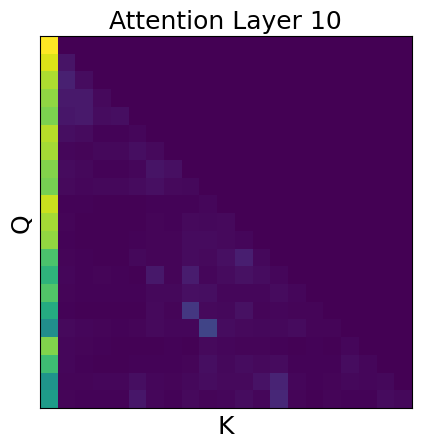
\includegraphics[width=0.85\columnwidth]{figures/obs4_no_intervention.png}
    \caption{No intervention}
    \label{fig:no_intervention}
  \end{subfigure}
  \begin{subfigure}[t]{0.22\textwidth}
    \centering
    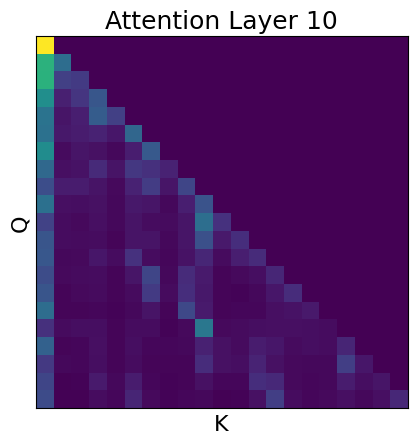
\includegraphics[width=0.85\columnwidth]{figures/obs4_intervention1.png}
    \caption{ nullify $b_Q$}
    \label{fig:intervention1}
  \end{subfigure}
  \begin{subfigure}[t]{0.22\textwidth}
    \centering
    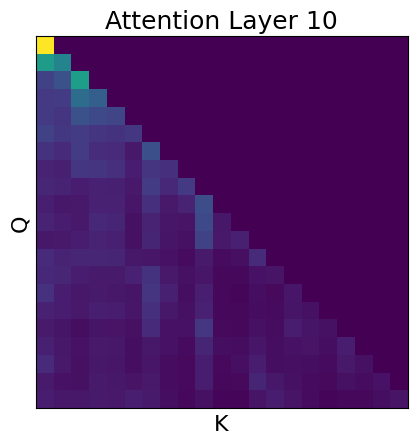
\includegraphics[width=0.85\columnwidth]{figures/obs4_intervention2.png}
    \caption{remove first EPE}
    \label{fig:intervention2}
  \end{subfigure}
  \begin{subfigure}[t]{0.22\textwidth}
    \centering
    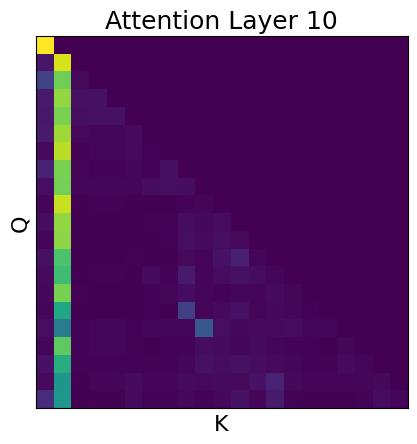
\includegraphics[width=0.85\columnwidth]{figures/obs4_intervention3.png}
    \caption{move first EPE}
    \label{fig:intervention3}
  \end{subfigure}
  \begin{subfigure}[t]{0.22\textwidth}
    \centering
    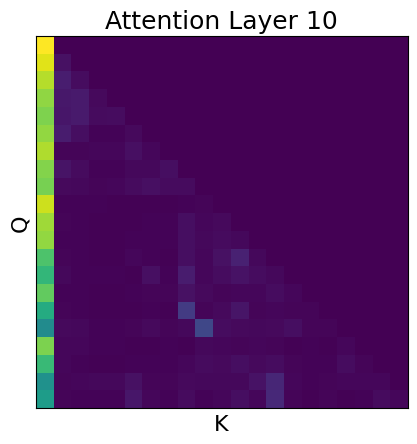
\includegraphics[width=0.85\columnwidth]{figures/obs4_intervention4.png}
    \caption{nullify BOS}
    \label{fig:intervention4}
  \end{subfigure}
  \begin{subfigure}[t]{0.22\textwidth}
    \centering
    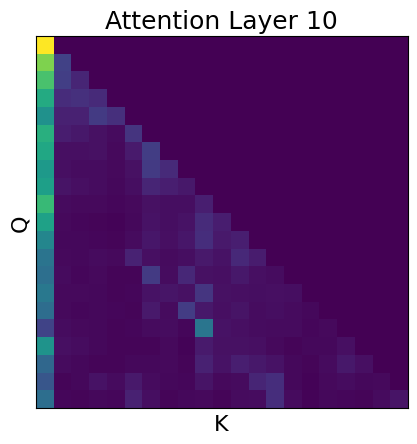
\includegraphics[width=0.85\columnwidth]{figures/obs4_intervention5.png}
    \caption{nullify massive activation columns of Wk}
    \label{fig:intervention5}
  \end{subfigure}
    \begin{subfigure}[t]{0.22\textwidth}
    \centering
    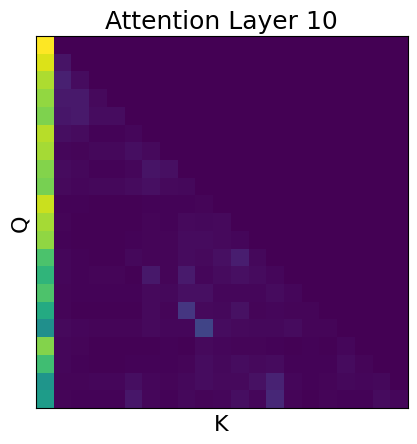
\includegraphics[width=0.85\columnwidth]{figures/obs4_intervention5_2.png}
    \caption{nullify random columns of Wk}
    \label{fig:intervention5_2}
  \end{subfigure}

  \caption{Comparison of attention maps under different interventions. (a) no intervention; (b) intervention 1: nullify $b_Q$; (c) intervention 2: remove the learned EPE at position 1 and add a different EPE (the second); (d) intervention 3: transplant the learned EPE to another position (the second). (e) intervention 4: nullify BOS token embedding. intervention 5: (f) nullify massive activation columns of Wk. (g) nullify random columns of Wk. \YRM{this is absolutely great, but *must* take up less space. Is there a way to make it smaller without hurting too much? (just making the pic smaller will make the x and y text too small, so we need something more delicate)}} 
  \label{fig:interventions_comparison}
\end{figure*}



\section{Conclusions}
Attention sinks are not universal. In architectures with learned query biases and absolute positional encodings, our analyses and interventions indicate that the sink is implemented through an interaction between (i) a learned query bias, (ii) the first-layer transformation of positional information that yields a high-magnitude effective positional encoding at the first position (EPE$_1$), and (iii) structure in the key projection aligned with the large-magnitude coordinates of EPE$_1$. Together with observations of sinks in models without these components (e.g with alternative positional schemes (e.g., RoPE or ALiBi; \YRM{cite}) or without a learned query bias \YRM{cite}), these results argue against a single universal mechanism for attention sink

\paragraph{Implications}
The lack of a single universal mechanism for attention sink hints that attention sink are an optimization-friendly attractor rather than a single architectural quirk: when multiple representational routes are available, training can discover a circuit that implements a sink. Consequently, naive, component-wise regularization is unlikely to eliminate the phenomenon—penalizing one element (e.g., shrinking the query bias) can be absorbed by alternative pathways. We offer these findings as a basis for developing and evaluating mitigations.



\section{Limitations}

\subsection{Scope across architectures and scales}
Our analyses focus on a GPT-2–style model with learned query biases and absolute positional encodings. The broader Transformer ecosystem includes architectures that omit such biases or use alternative positional schemes (e.g., RoPE, ALiBi). We do not establish whether the same circuit forms in those settings, nor whether the EPE–$W_k$–$b_Q$ interaction generalizes unchanged. In addition, GPT-2 is small by contemporary standards; with scale, the mechanism could strengthen, fragment into multiple pathways, or be replaced by different circuits.

\subsection{Learning dynamics}
We provide a post-hoc, static analysis of a trained checkpoint. We do not track when the circuit emerges during pre-training, which gradients give rise to it, or whether intermediate snapshots exhibit qualitatively different pathways. Train-time causality—e.g., whether specific regularizers prevent the circuit from forming—remains outside our scope.

\subsection{Mechanism vs. function}
Our contribution is mechanistic: we explain \emph{how} an attention sink can be implemented in the studied architecture. We do not claim a definitive \emph{functional} rationale for \emph{why} such a sink is beneficial or harmful across tasks. Establishing the downstream utility or cost of the sink, and the conditions under which it is selected by optimization, is left for future work.



% Use ACL bibliography style / file
\bibliographystyle{acl_natbib}
\bibliography{latex/custom}

\appendix

\section{}\label{app:bias_term}

\begin{figure*}[t]
  \begin{subfigure}[t]{0.24\textwidth}
    \centering
    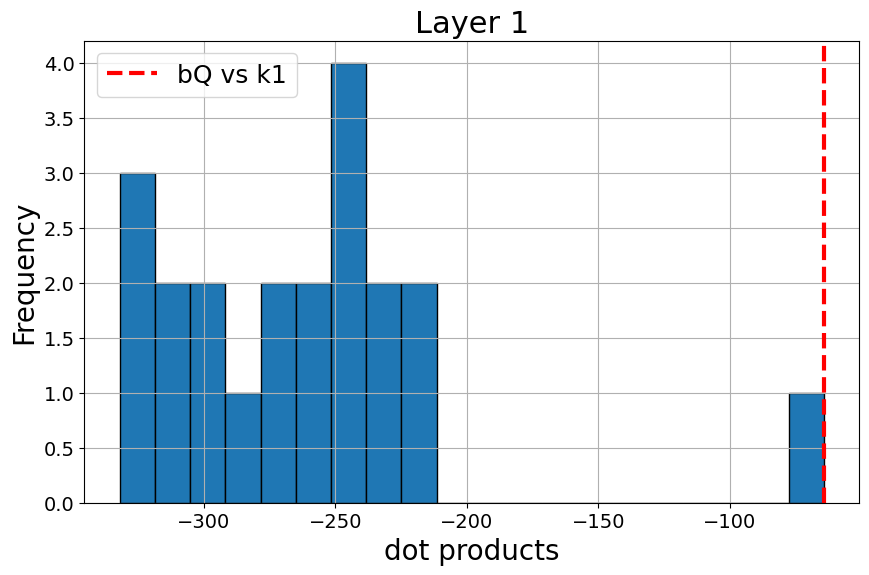
\includegraphics[width=1.4\columnwidth]{figures/obs1_appendix/obs1_layer1.png}
    \caption{layer 1}
  \end{subfigure}\hfill
  \begin{subfigure}[t]{0.24\textwidth}
    \centering
    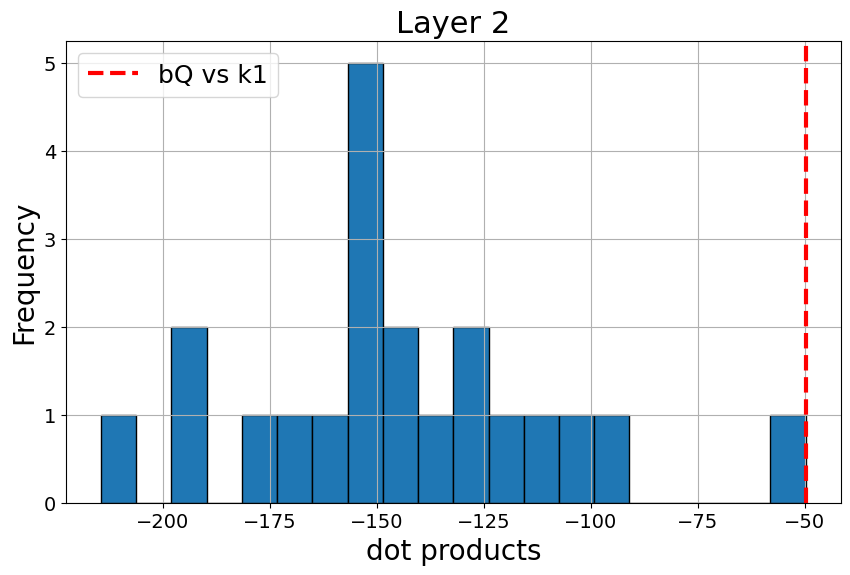
\includegraphics[width=1.4\columnwidth]{figures/obs1_appendix/obs1_layer2.png}
    \caption{layer 2}
  \end{subfigure}\hfill
  \begin{subfigure}[t]{0.24\textwidth}
    \centering
    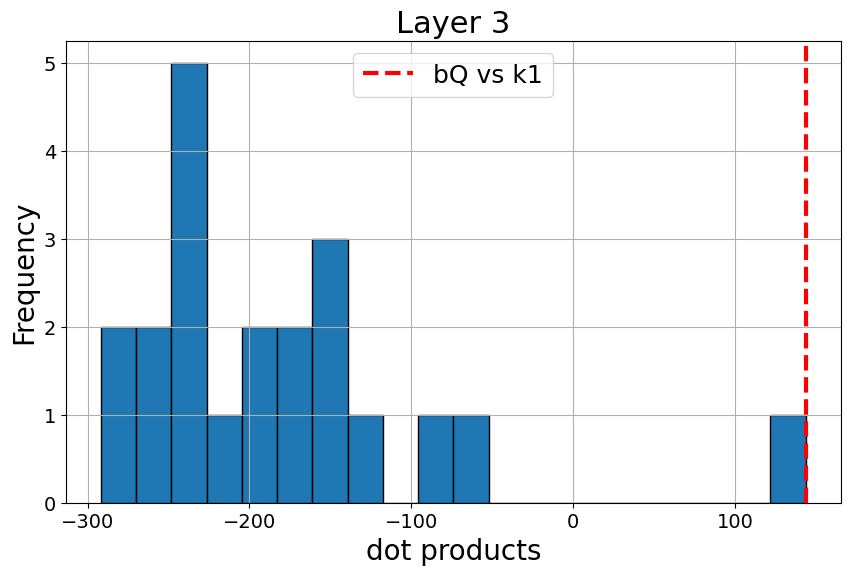
\includegraphics[width=1.4\columnwidth]{figures/obs1_appendix/obs1_layer3.png}
    \caption{layer 3}
  \end{subfigure}\hfill
    \vspace{2mm}

  \begin{subfigure}[t]{0.24\textwidth}
    \centering
    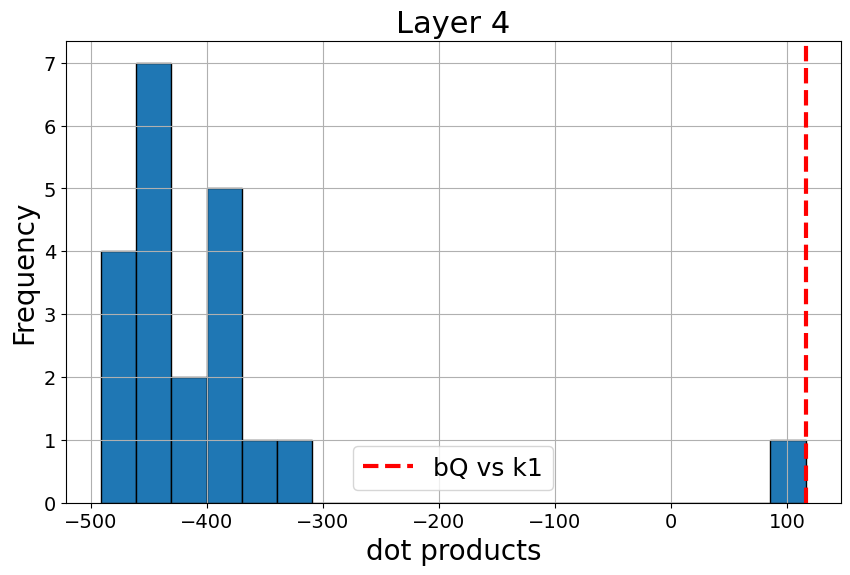
\includegraphics[width=1.4\columnwidth]{figures/obs1_appendix/obs1_layer4.png}
    \caption{layer 4}
  \end{subfigure}\hfill
  \begin{subfigure}[t]{0.24\textwidth}
    \centering
    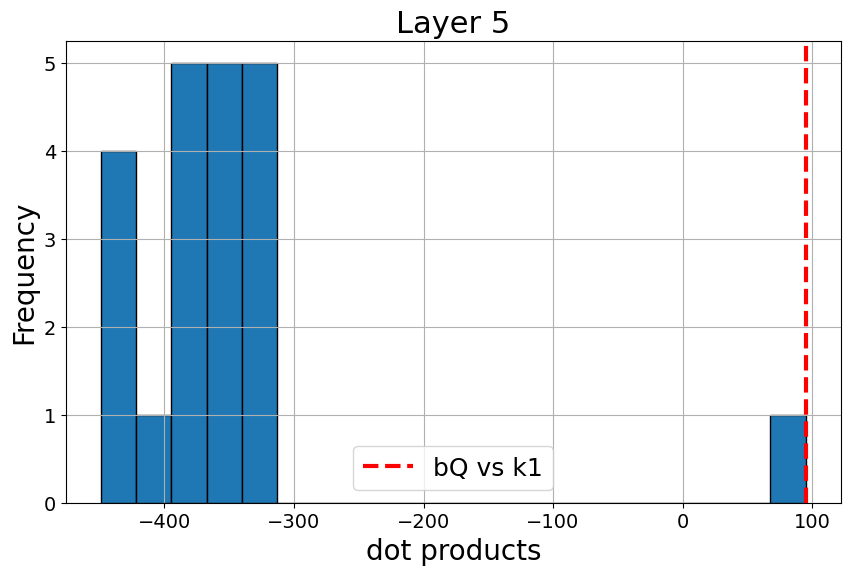
\includegraphics[width=1.4\columnwidth]{figures/obs1_appendix/obs1_layer5.png}
    \caption{layer 5}
  \end{subfigure}\hfill
  \begin{subfigure}[t]{0.24\textwidth}
    \centering
    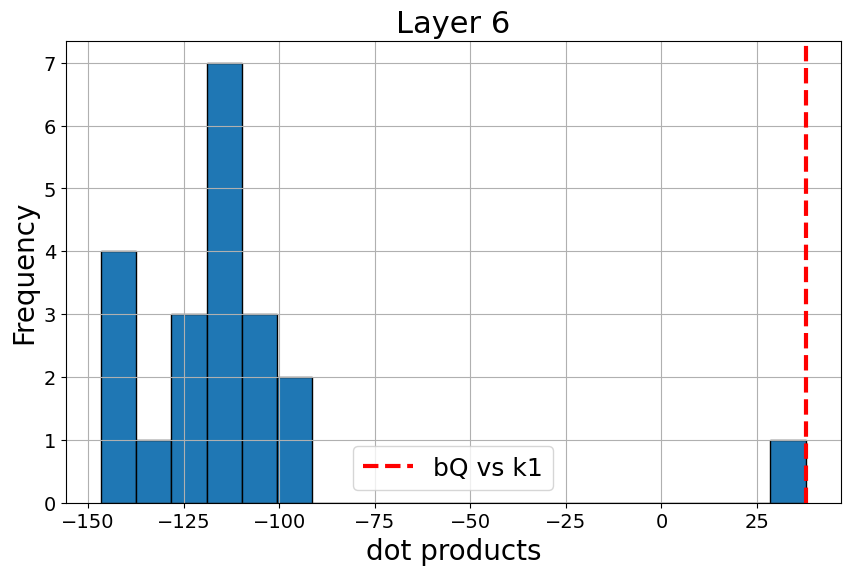
\includegraphics[width=1.4\columnwidth]{figures/obs1_appendix/obs1_layer6.png}
    \caption{layer 6}
  \end{subfigure}\hfill
    \vspace{2mm}

    \begin{subfigure}[t]{0.24\textwidth}
    \centering
    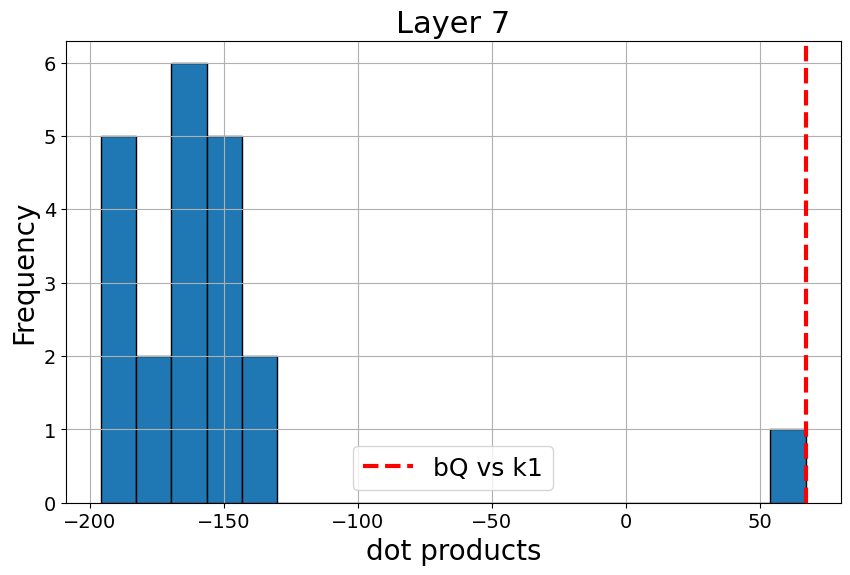
\includegraphics[width=1.4\columnwidth]{figures/obs1_appendix/obs1_layer7.png}
    \caption{layer 7}
  \end{subfigure}\hfill
      \begin{subfigure}[t]{0.24\textwidth}
    \centering
    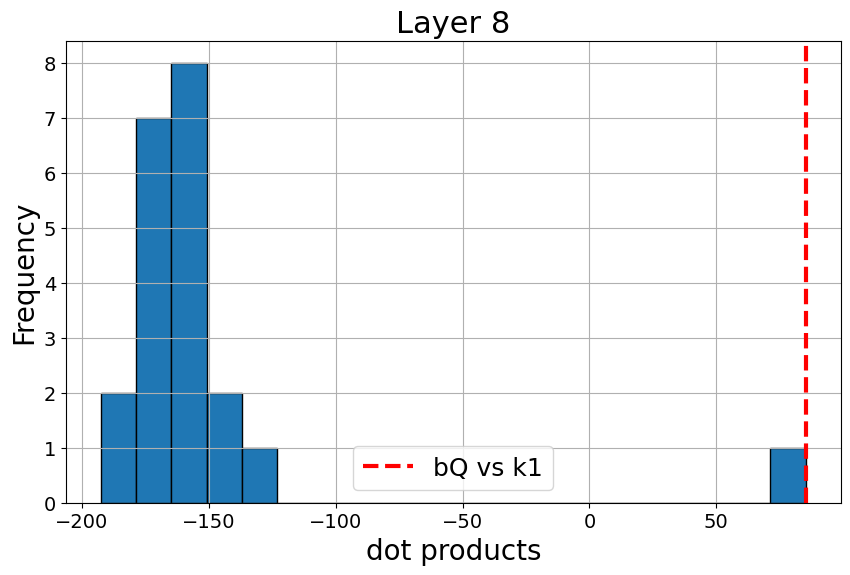
\includegraphics[width=1.4\columnwidth]{figures/obs1_appendix/obs1_layer8.png}
    \caption{layer 8}
  \end{subfigure}\hfill
      \begin{subfigure}[t]{0.24\textwidth}
    \centering
    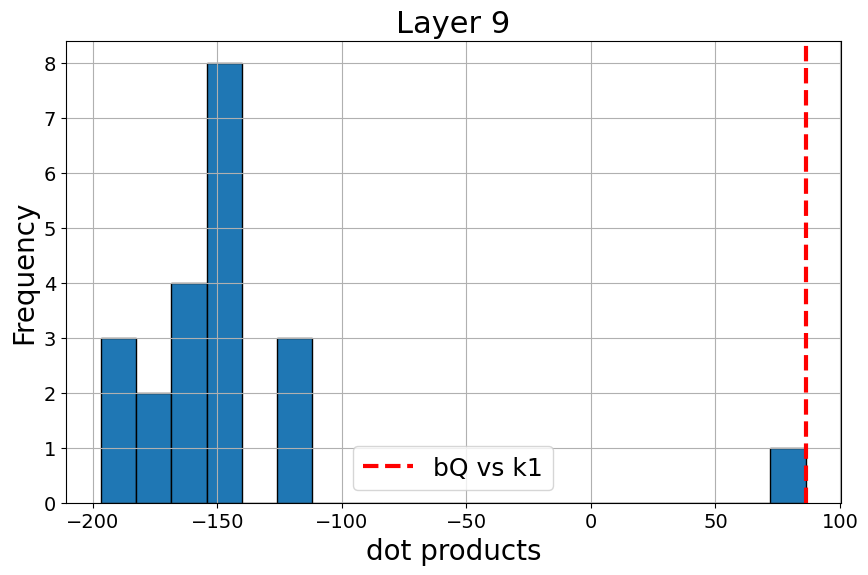
\includegraphics[width=1.4\columnwidth]{figures/obs1_appendix/obs1_layer9.png}
    \caption{layer 9}
  \end{subfigure}\hfill
    \vspace{2mm}
    
    \begin{subfigure}[t]{0.24\textwidth}
    \centering
    \includegraphics[width=1.4\columnwidth]{figures/obs1_appendix/obs1_layer10.png}
    \caption{layer 10}
  \end{subfigure}\hfill
    \begin{subfigure}[t]{0.24\textwidth}
    \centering
    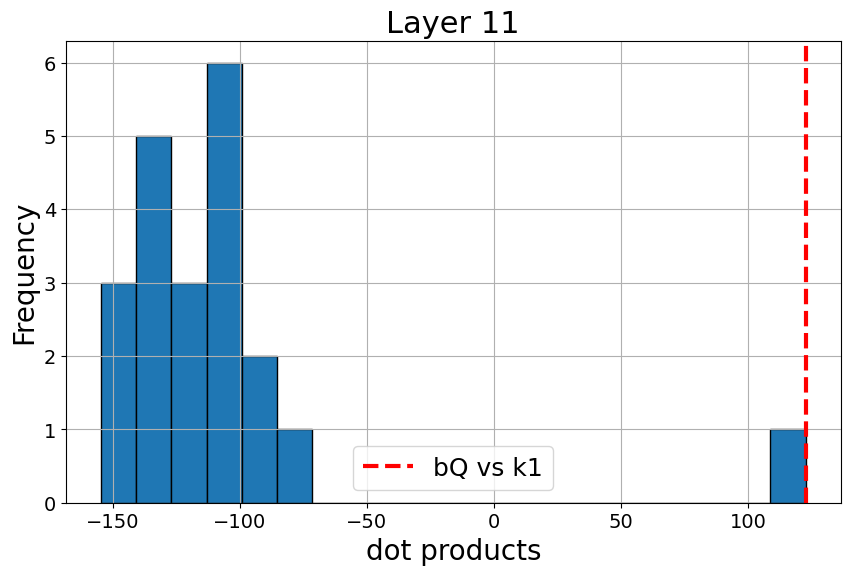
\includegraphics[width=1.4\columnwidth]{figures/obs1_appendix/obs1_layer11.png}
    \caption{layer 11}
  \end{subfigure}\hfill
  \begin{subfigure}[t]{0.24\textwidth}
    \centering
    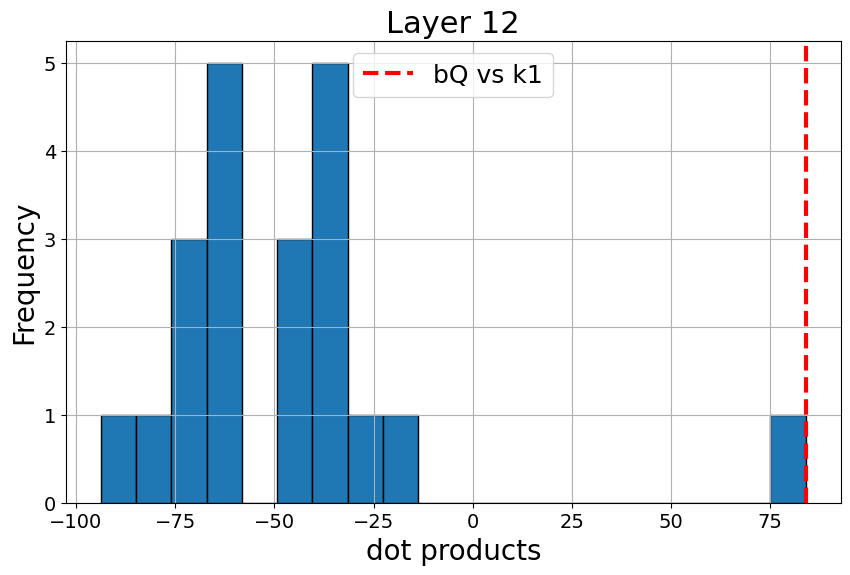
\includegraphics[width=1.4\columnwidth]{figures/obs1_appendix/obs1_layer12.png}
    \caption{layer 12}
  \end{subfigure}\hfill
    \vspace{2mm}
  \caption{Distribution of bias terms $\Delta_j^$ across positions for all of the layers}
\end{figure*}

\section{}\label{app:epe_bias}

\begin{figure*}[t]
  \begin{subfigure}[t]{0.24\textwidth}
    \centering
    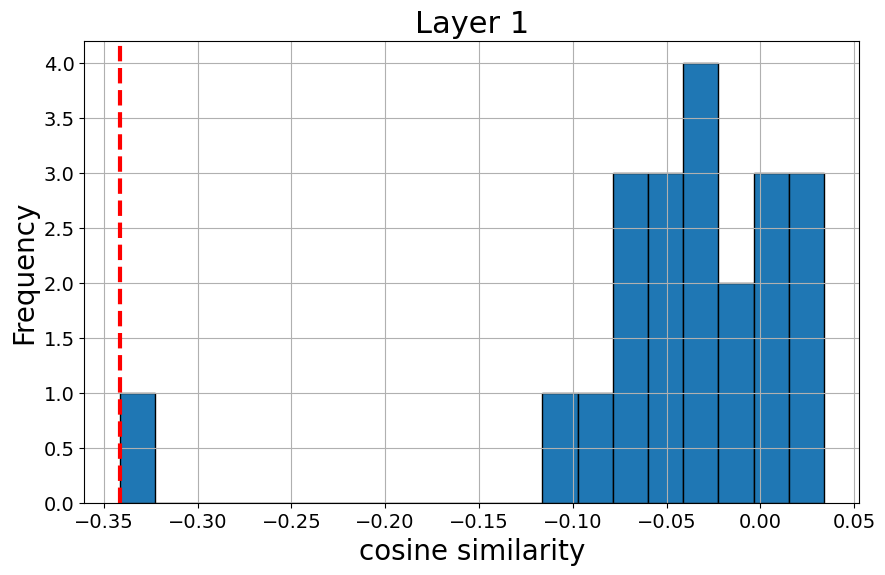
\includegraphics[width=1.4\columnwidth]{figures/obs2_appendix/obs2_layer1.png}
    \caption{layer 1}
  \end{subfigure}\hfill
  \begin{subfigure}[t]{0.24\textwidth}
    \centering
    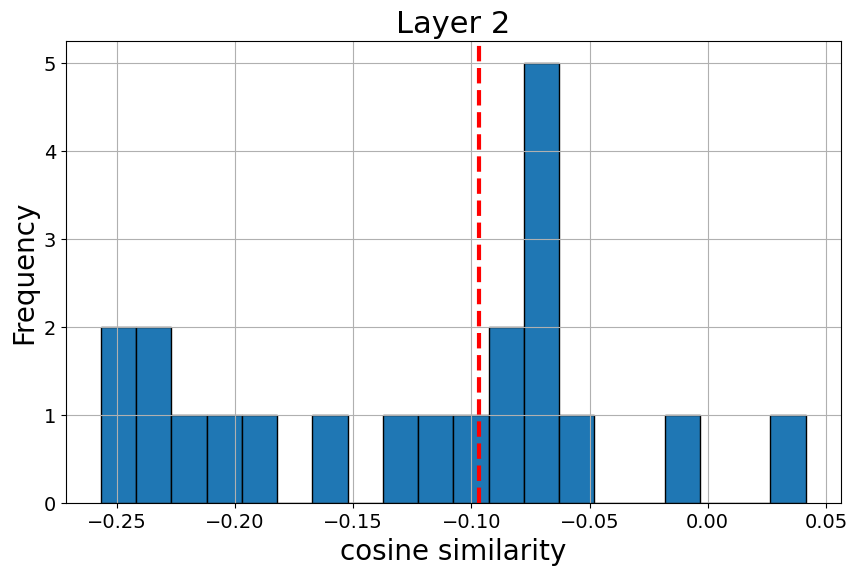
\includegraphics[width=1.4\columnwidth]{figures/obs2_appendix/obs2_layer2.png}
    \caption{layer 2}
  \end{subfigure}\hfill
  \begin{subfigure}[t]{0.24\textwidth}
    \centering
    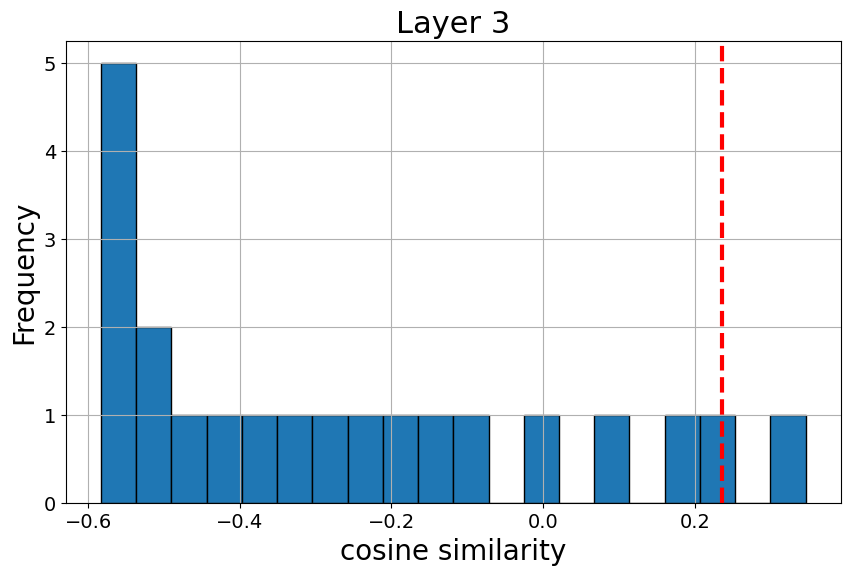
\includegraphics[width=1.4\columnwidth]{figures/obs2_appendix/obs2_layer3.png}
    \caption{layer 3}
  \end{subfigure}\hfill
    \vspace{2mm}

  \begin{subfigure}[t]{0.24\textwidth}
    \centering
    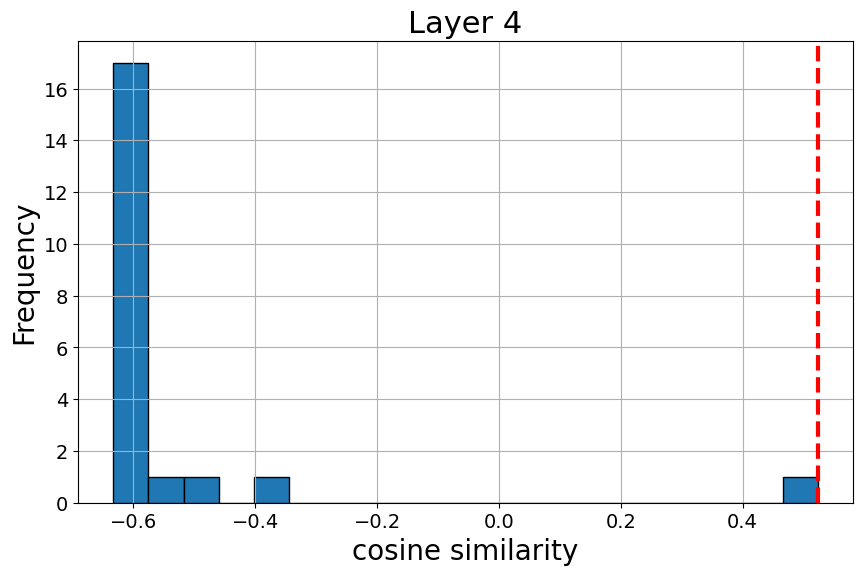
\includegraphics[width=1.4\columnwidth]{figures/obs2_appendix/obs2_layer4.png}
    \caption{layer 4}
  \end{subfigure}\hfill
  \begin{subfigure}[t]{0.24\textwidth}
    \centering
    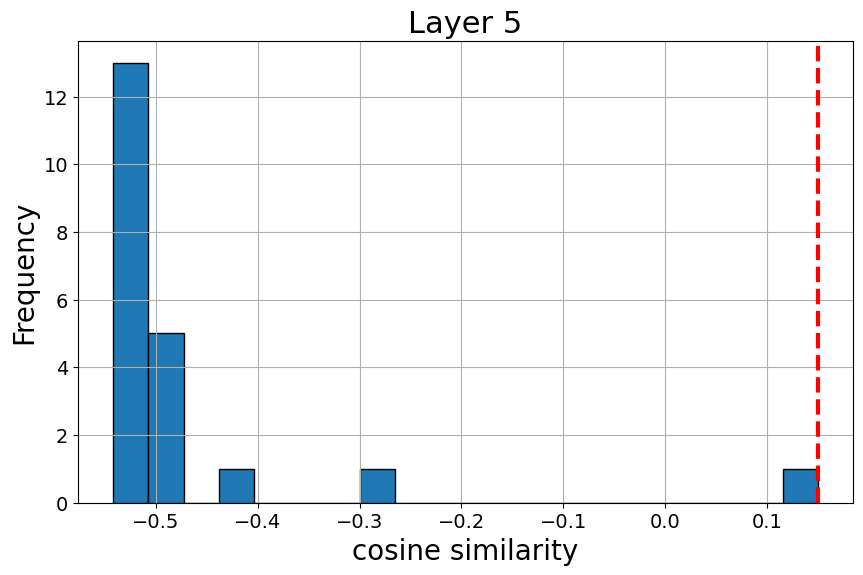
\includegraphics[width=1.4\columnwidth]{figures/obs2_appendix/obs2_layer5.png}
    \caption{layer 5}
  \end{subfigure}\hfill
  \begin{subfigure}[t]{0.24\textwidth}
    \centering
    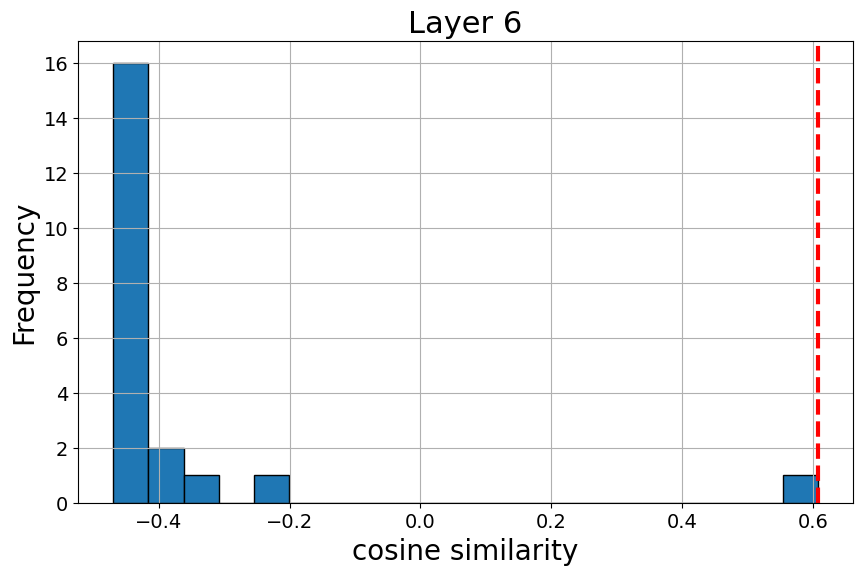
\includegraphics[width=1.4\columnwidth]{figures/obs2_appendix/obs2_layer6.png}
    \caption{layer 6}
  \end{subfigure}\hfill
    \vspace{2mm}

    \begin{subfigure}[t]{0.24\textwidth}
    \centering
    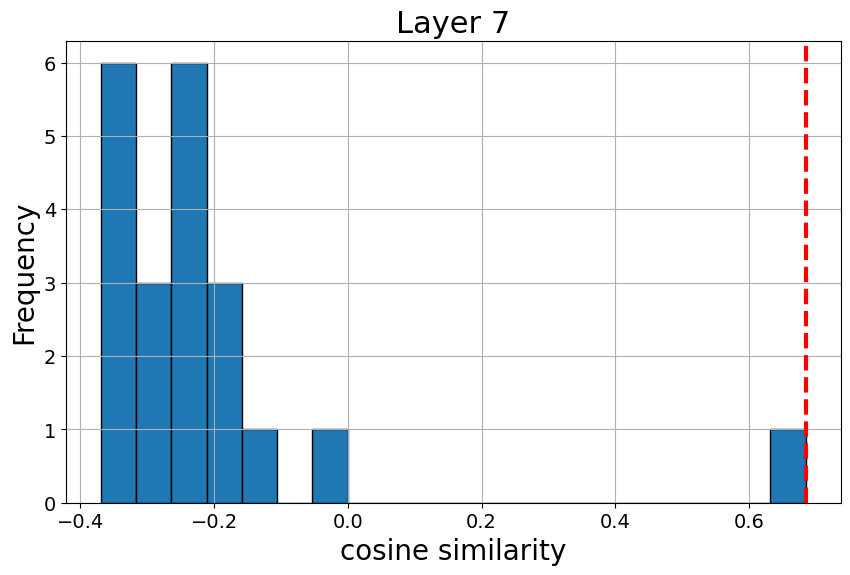
\includegraphics[width=1.4\columnwidth]{figures/obs2_appendix/obs2_layer7.png}
    \caption{layer 7}
  \end{subfigure}\hfill
      \begin{subfigure}[t]{0.24\textwidth}
    \centering
    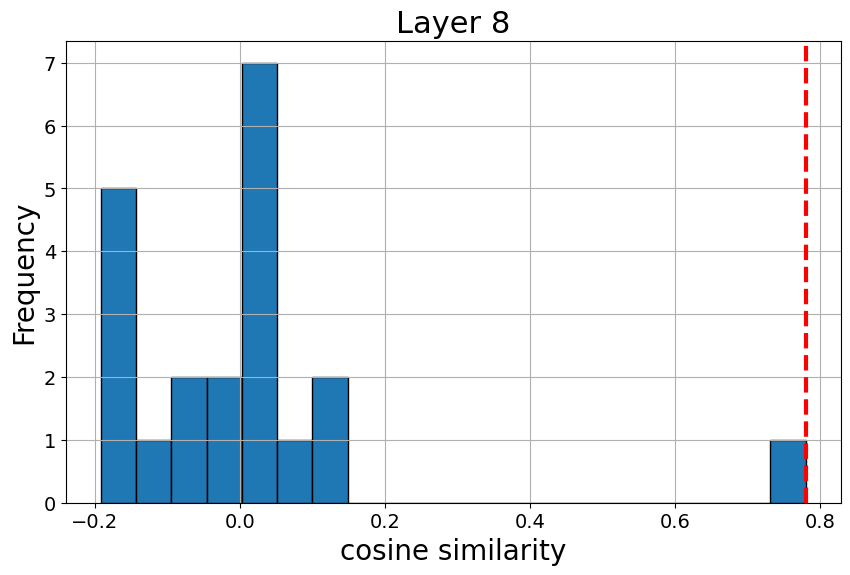
\includegraphics[width=1.4\columnwidth]{figures/obs2_appendix/obs2_layer8.png}
    \caption{layer 8}
  \end{subfigure}\hfill
      \begin{subfigure}[t]{0.24\textwidth}
    \centering
    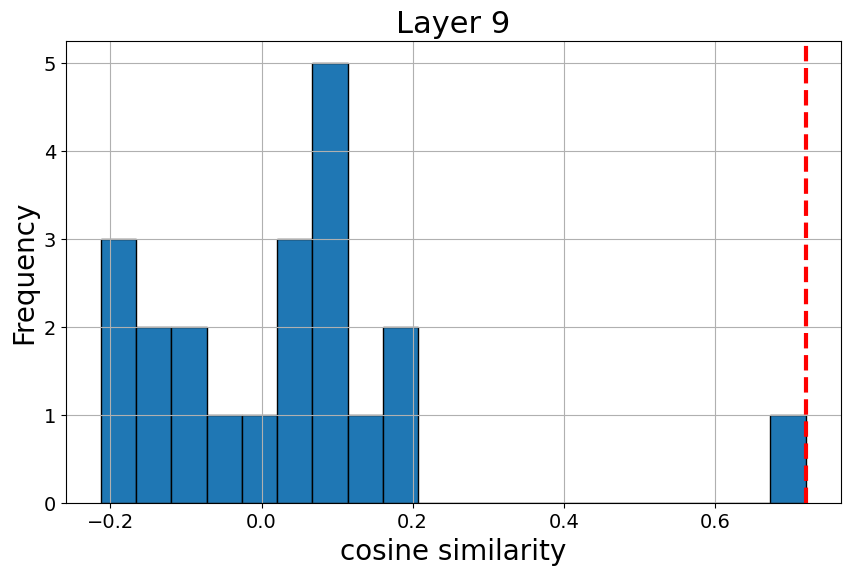
\includegraphics[width=1.4\columnwidth]{figures/obs2_appendix/obs2_layer9.png}
    \caption{layer 9}
  \end{subfigure}\hfill
    \vspace{2mm}
    
    \begin{subfigure}[t]{0.24\textwidth}
    \centering
    \includegraphics[width=1.4\columnwidth]{figures/obs2_appendix/obs2_layer10.png}
    \caption{layer 10}
  \end{subfigure}\hfill
    \begin{subfigure}[t]{0.24\textwidth}
    \centering
    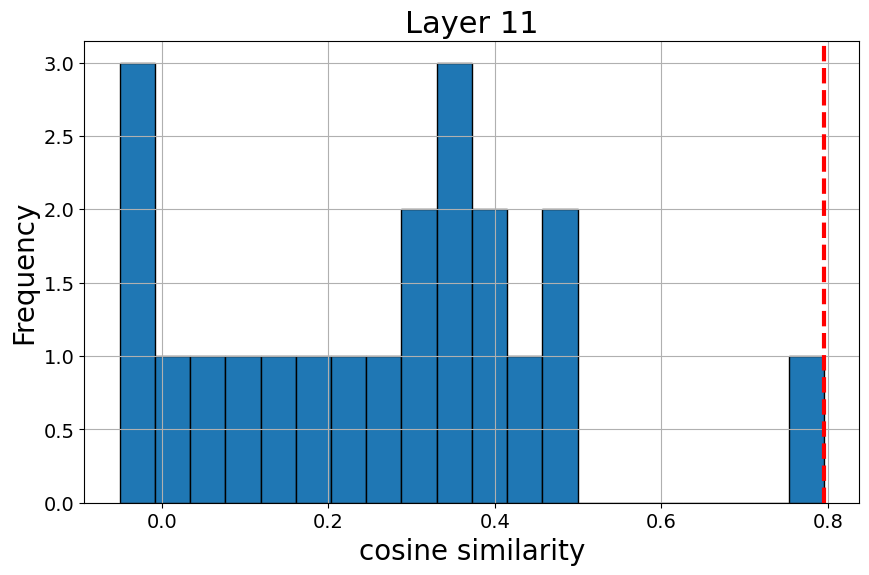
\includegraphics[width=1.4\columnwidth]{figures/obs2_appendix/obs2_layer11.png}
    \caption{layer 11}
  \end{subfigure}\hfill
  \begin{subfigure}[t]{0.24\textwidth}
    \centering
    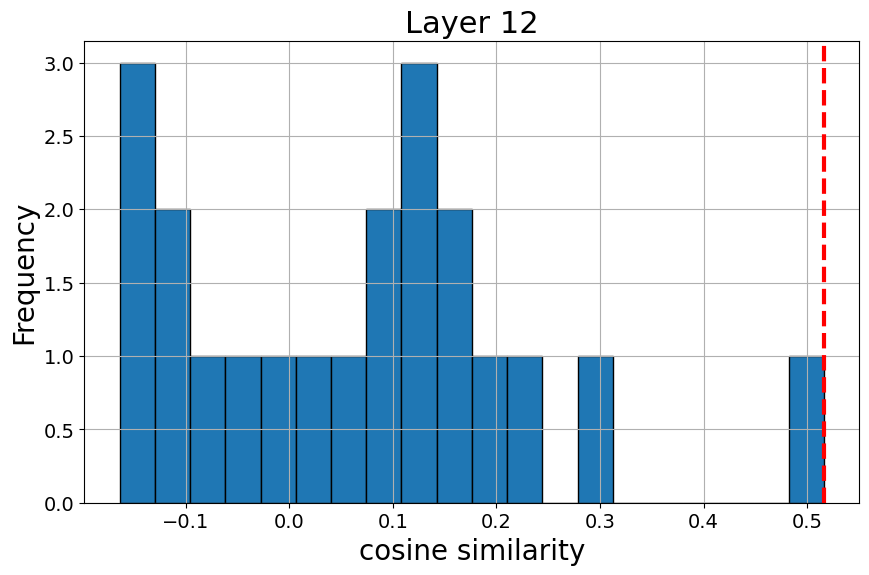
\includegraphics[width=1.4\columnwidth]{figures/obs2_appendix/obs2_layer12.png}
    \caption{layer 12}
  \end{subfigure}\hfill
    \vspace{2mm}

  \caption{Cosine similarity between query bias $b_Q^{(10)}$ and $W_k^{(10)}\mathrm{EPE}$.}
\end{figure*}

\section{}\label{app:massive_activations_in_ppe}

\begin{figure}[t]
  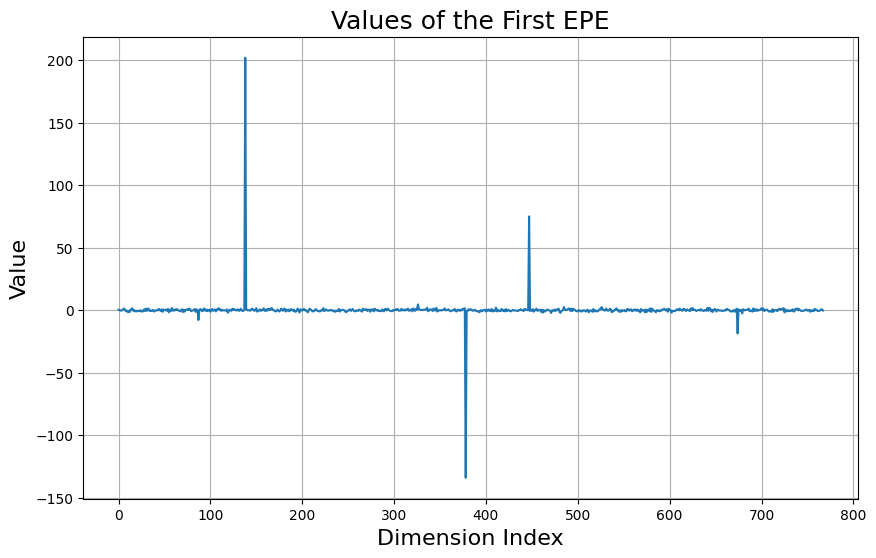
\includegraphics[width=\columnwidth]{figures/massive_activations_in_ppe.png}
  \caption{Values of the $\mathrm{EPE}_1$ vector for the first token. Most coordinates remain near zero, but a small number exhibit extremely large positive or negative magnitudes, which we refer to as ``massive activations.'' These amplified dimensions are the ones later aligned with $W_k$ and $b_Q$ in our analysis.}
\end{figure}

\section{} \label{app:coor_align}
\begin{table}[t]
  \centering
  \begin{tabular}{llll}
    \hline
    \textbf{Layer} & \textbf{Baseline} & \textbf{$d{=}138$} & \textbf{$d{=}447$}\\
    \hline
    layer 1   &   4.47$\pm$22.226     &    12.116   &    11.064        \\
    layer 2   &   2.8$\pm$6.62    &    8.065   &    24.468         \\
    layer 3   &   1.717$\pm$5.826 &    10.178  &    23.047        \\
    layer 4   &   1.657$\pm$5.02  &   18.198   &     17.149         \\
    layer 5   &   1.561$\pm$4.618 &    3.072   &    23.854          \\
    layer 6   &   0.86$\pm$1.59   &    5.644   &    6.142          \\
    layer 8   &   1.404$\pm$3.546 &    19.806  &    28.01          \\
    layer 10  &   1.313$\pm$3.616 &    23.131  &    28.42        \\
    layer 12   &   1.145$\pm$2.65 &    4.5  &    13.59         \\

    \hline
  \end{tabular}
  \caption{$\gamma^{(i)}=(W_k^{(i)})^\top b_Q^{(i)}$ at coordinates where $\mathrm{EPE}_1$ has massive activations (dims 138, 447) versus the mean of all of the columns. Massive-$\mathrm{EPE}_1$ coordinates have substantially higher values across layers, confirming that $\mathrm{EPE}_1$ is large exactly where the bias projection is large.}
\end{table}

\section{}\label{app:interventions}

\subsection{}\label{app:no_intervention}
\begin{figure*}[t]
  \begin{subfigure}[t]{0.24\textwidth}
    \centering
    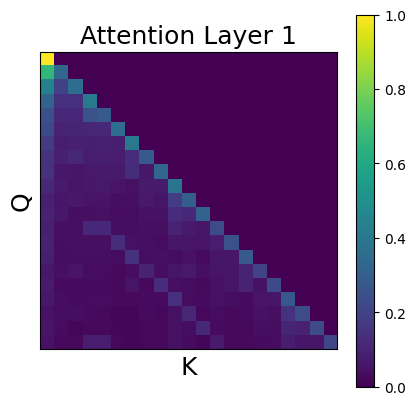
\includegraphics[width=1.4\columnwidth]{figures/no_intervention/layer_1.png}
    \caption{layer 1}
  \end{subfigure}\hfill
  \begin{subfigure}[t]{0.24\textwidth}
    \centering
    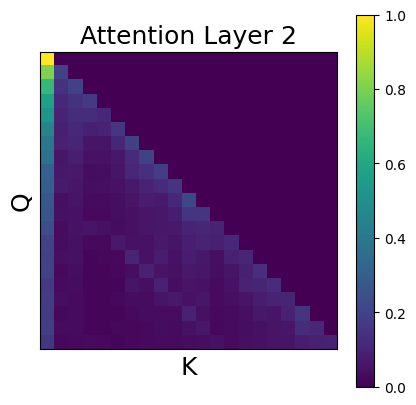
\includegraphics[width=1.4\columnwidth]{figures/no_intervention/layer_2.png}
    \caption{layer 2}
  \end{subfigure}\hfill
  \begin{subfigure}[t]{0.24\textwidth}
    \centering
    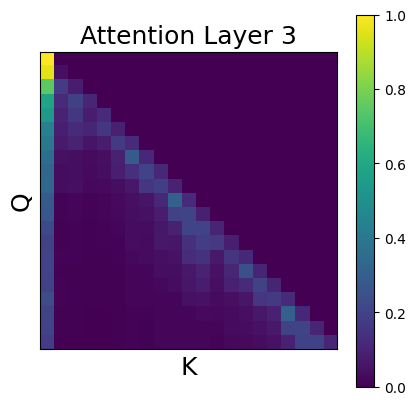
\includegraphics[width=1.4\columnwidth]{figures/no_intervention/layer_3.png}
    \caption{layer 3}
  \end{subfigure}\hfill

  \begin{subfigure}[t]{0.24\textwidth}
    \centering
    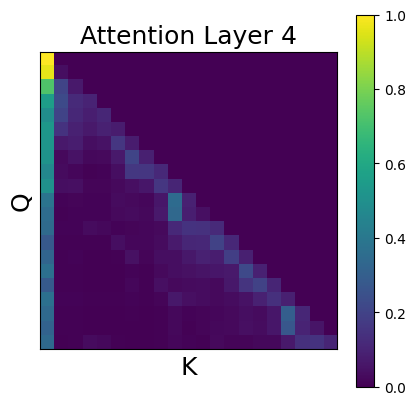
\includegraphics[width=1.4\columnwidth]{figures/no_intervention/layer_4.png}
    \caption{layer 4}
  \end{subfigure}\hfill
  \begin{subfigure}[t]{0.24\textwidth}
    \centering
    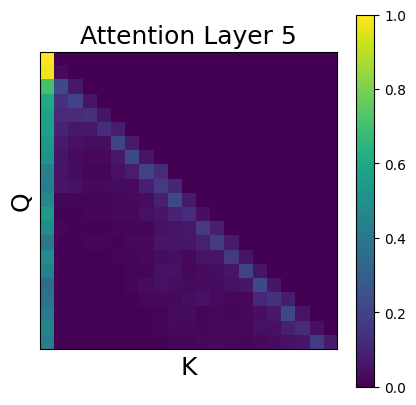
\includegraphics[width=1.4\columnwidth]{figures/no_intervention/layer_5.png}
    \caption{layer 5}
  \end{subfigure}\hfill
  \begin{subfigure}[t]{0.24\textwidth}
    \centering
    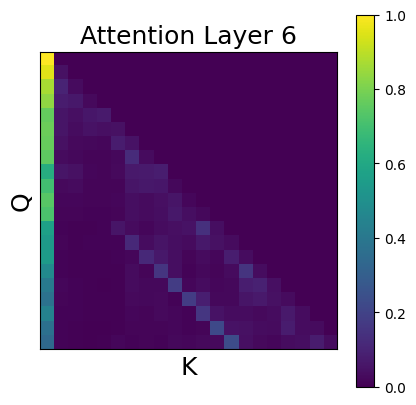
\includegraphics[width=1.4\columnwidth]{figures/no_intervention/layer_6.png}
    \caption{layer 6}
  \end{subfigure}\hfill

    \begin{subfigure}[t]{0.24\textwidth}
    \centering
    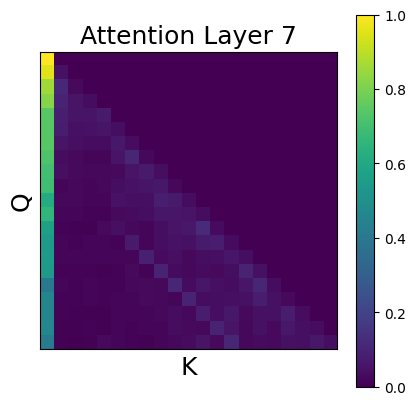
\includegraphics[width=1.4\columnwidth]{figures/no_intervention/layer_7.png}
    \caption{layer 7}
  \end{subfigure}\hfill
      \begin{subfigure}[t]{0.24\textwidth}
    \centering
    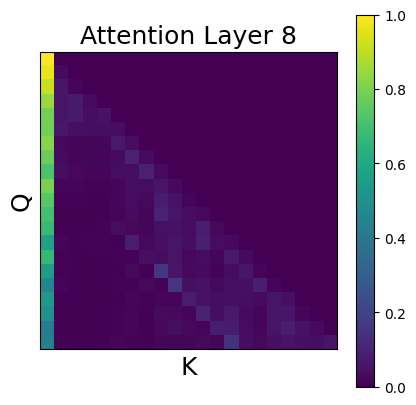
\includegraphics[width=1.4\columnwidth]{figures/no_intervention/layer_8.png}
    \caption{layer 8}
  \end{subfigure}\hfill
      \begin{subfigure}[t]{0.24\textwidth}
    \centering
    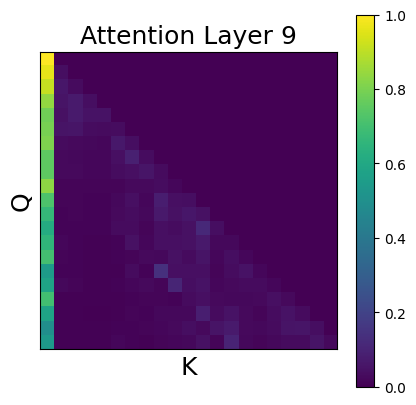
\includegraphics[width=1.4\columnwidth]{figures/no_intervention/layer_9.png}
    \caption{layer 9}
  \end{subfigure}\hfill
    
    \begin{subfigure}[t]{0.24\textwidth}
    \centering
    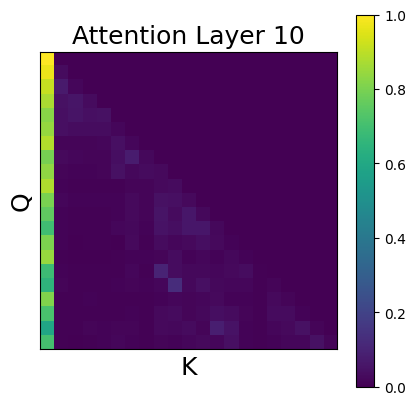
\includegraphics[width=1.4\columnwidth]{figures/no_intervention/layer_10.png}
    \caption{layer 10}
  \end{subfigure}\hfill
    \begin{subfigure}[t]{0.24\textwidth}
    \centering
    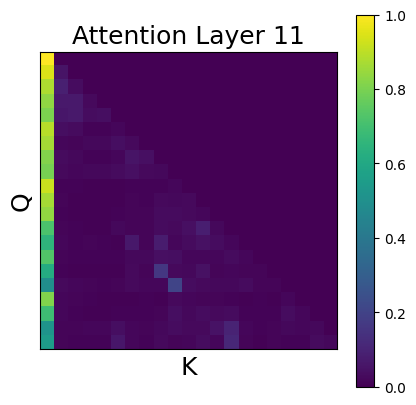
\includegraphics[width=1.4\columnwidth]{figures/no_intervention/layer_11.png}
    \caption{layer 11}
  \end{subfigure}\hfill
  \begin{subfigure}[t]{0.24\textwidth}
    \centering
    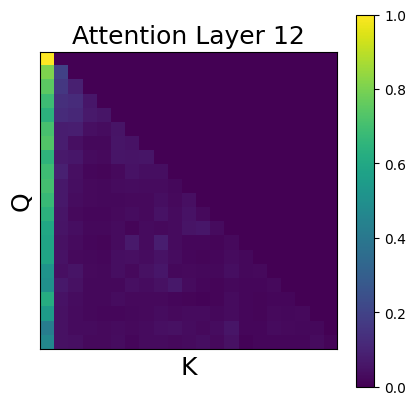
\includegraphics[width=1.4\columnwidth]{figures/no_intervention/layer_12.png}
    \caption{layer 12}
  \end{subfigure}\hfill

  \caption{Attention maps for all layers with no intervention. There is a visible attention sink in most layers}
\end{figure*}


\subsection{}\label{app:intervention1}
\begin{figure*}[t]
  \begin{subfigure}[t]{0.24\textwidth}
    \centering
    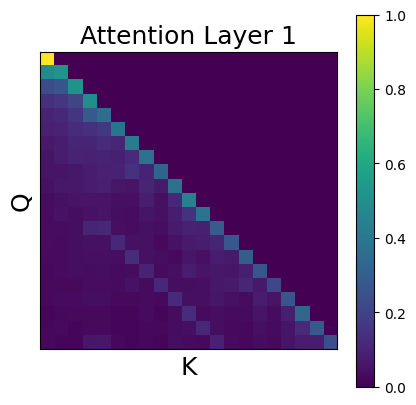
\includegraphics[width=1.4\columnwidth]{figures/intervention1/layer_1.png}
    \caption{layer 1}
  \end{subfigure}\hfill
  \begin{subfigure}[t]{0.24\textwidth}
    \centering
    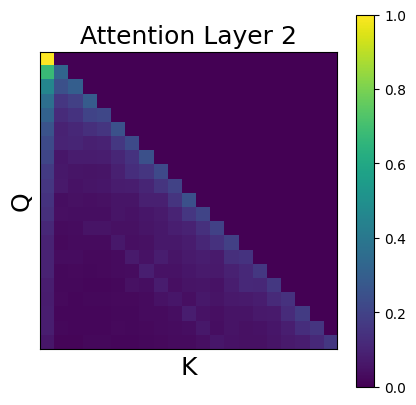
\includegraphics[width=1.4\columnwidth]{figures/intervention1/layer_2.png}
    \caption{layer 2}
  \end{subfigure}\hfill
  \begin{subfigure}[t]{0.24\textwidth}
    \centering
    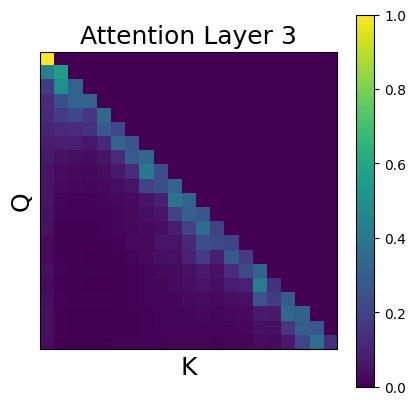
\includegraphics[width=1.4\columnwidth]{figures/intervention1/layer_3.png}
    \caption{layer 3}
  \end{subfigure}\hfill

  \begin{subfigure}[t]{0.24\textwidth}
    \centering
    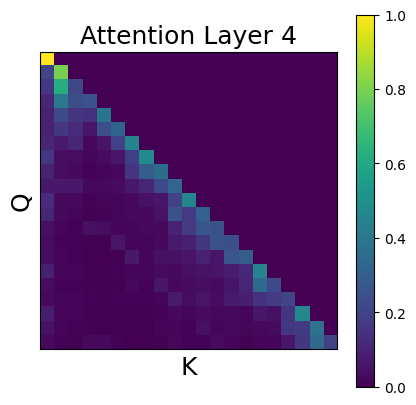
\includegraphics[width=1.4\columnwidth]{figures/intervention1/layer_4.png}
    \caption{layer 4}
  \end{subfigure}\hfill
  \begin{subfigure}[t]{0.24\textwidth}
    \centering
    \includegraphics[width=1.4\columnwidth]{figures/intervention1/layer_5.png}
    \caption{layer 5}
  \end{subfigure}\hfill
  \begin{subfigure}[t]{0.24\textwidth}
    \centering
    \includegraphics[width=1.4\columnwidth]{figures/intervention1/layer_6.png}
    \caption{layer 6}
  \end{subfigure}\hfill

    \begin{subfigure}[t]{0.24\textwidth}
    \centering
    \includegraphics[width=1.4\columnwidth]{figures/intervention1/layer_7.png}
    \caption{layer 7}
  \end{subfigure}\hfill
      \begin{subfigure}[t]{0.24\textwidth}
    \centering
    \includegraphics[width=1.4\columnwidth]{figures/intervention1/layer_8.png}
    \caption{layer 8}
  \end{subfigure}\hfill
      \begin{subfigure}[t]{0.24\textwidth}
    \centering
    \includegraphics[width=1.4\columnwidth]{figures/intervention1/layer_9.png}
    \caption{layer 9}
  \end{subfigure}\hfill
    
    \begin{subfigure}[t]{0.24\textwidth}
    \centering
    \includegraphics[width=1.4\columnwidth]{figures/intervention1/layer_10.png}
    \caption{layer 10}
  \end{subfigure}\hfill
    \begin{subfigure}[t]{0.24\textwidth}
    \centering
    \includegraphics[width=1.4\columnwidth]{figures/intervention1/layer_11.png}
    \caption{layer 11}
  \end{subfigure}\hfill
  \begin{subfigure}[t]{0.24\textwidth}
    \centering
    \includegraphics[width=1.4\columnwidth]{figures/intervention1/layer_12.png}
    \caption{layer 12}
  \end{subfigure}\hfill

  \caption{Intervention 1: Attention maps for all layers with nullufying $b_Q$. The attention sink is significantly resuced across layers}
\end{figure*}


\subsection{}\label{app:intervention2}
\begin{figure*}[t]
  \begin{subfigure}[t]{0.24\textwidth}
    \centering
    \includegraphics[width=1.4\columnwidth]{figures/intervention2/layer_1.png}
    \caption{layer 1}
  \end{subfigure}\hfill
  \begin{subfigure}[t]{0.24\textwidth}
    \centering
    \includegraphics[width=1.4\columnwidth]{figures/intervention2/layer_2.png}
    \caption{layer 2}
  \end{subfigure}\hfill
  \begin{subfigure}[t]{0.24\textwidth}
    \centering
    \includegraphics[width=1.4\columnwidth]{figures/intervention2/layer_3.png}
    \caption{layer 3}
  \end{subfigure}\hfill

  \begin{subfigure}[t]{0.24\textwidth}
    \centering
    \includegraphics[width=1.4\columnwidth]{figures/intervention2/layer_4.png}
    \caption{layer 4}
    \label{fig:obs2_layer4}
  \end{subfigure}\hfill
  \begin{subfigure}[t]{0.24\textwidth}
    \centering
    \includegraphics[width=1.4\columnwidth]{figures/intervention2/layer_5.png}
    \caption{layer 5}
  \end{subfigure}\hfill
  \begin{subfigure}[t]{0.24\textwidth}
    \centering
    \includegraphics[width=1.4\columnwidth]{figures/intervention2/layer_6.png}
    \caption{layer 6}
  \end{subfigure}\hfill

    \begin{subfigure}[t]{0.24\textwidth}
    \centering
    \includegraphics[width=1.4\columnwidth]{figures/intervention2/layer_7.png}
    \caption{layer 7}
  \end{subfigure}\hfill
      \begin{subfigure}[t]{0.24\textwidth}
    \centering
    \includegraphics[width=1.4\columnwidth]{figures/intervention2/layer_8.png}
    \caption{layer 8}
  \end{subfigure}\hfill
      \begin{subfigure}[t]{0.24\textwidth}
    \centering
    \includegraphics[width=1.4\columnwidth]{figures/intervention2/layer_9.png}
    \caption{layer 9}
  \end{subfigure}\hfill
    
    \begin{subfigure}[t]{0.24\textwidth}
    \centering
    \includegraphics[width=1.4\columnwidth]{figures/intervention2/layer_10.png}
    \caption{layer 10}
  \end{subfigure}\hfill
    \begin{subfigure}[t]{0.24\textwidth}
    \centering
    \includegraphics[width=1.4\columnwidth]{figures/intervention2/layer_11.png}
    \caption{layer 11}
  \end{subfigure}\hfill
  \begin{subfigure}[t]{0.24\textwidth}
    \centering
    \includegraphics[width=1.4\columnwidth]{figures/intervention2/layer_12.png}
    \caption{layer 12}
  \end{subfigure}\hfill

  \caption{Intervention 2: Attention maps for all layers with swaping $\mathrm{EPE}_1$ with another position’s EPE; the first-position sink disappears}
\end{figure*}

\subsection{}\label{app:intervention3}
\begin{figure*}[t]
  \begin{subfigure}[t]{0.24\textwidth}
    \centering
    \includegraphics[width=1.4\columnwidth]{figures/intervention3/layer_1.png}
    \caption{layer 1}
  \end{subfigure}\hfill
  \begin{subfigure}[t]{0.24\textwidth}
    \centering
    \includegraphics[width=1.4\columnwidth]{figures/intervention3/layer_2.png}
    \caption{layer 2}
  \end{subfigure}\hfill
  \begin{subfigure}[t]{0.24\textwidth}
    \centering
    \includegraphics[width=1.4\columnwidth]{figures/intervention3/layer_3.png}
    \caption{layer 3}
  \end{subfigure}\hfill

  \begin{subfigure}[t]{0.24\textwidth}
    \centering
    \includegraphics[width=1.4\columnwidth]{figures/intervention3/layer_4.png}
    \caption{layer 4}
    \label{fig:obs2_layer4}
  \end{subfigure}\hfill
  \begin{subfigure}[t]{0.24\textwidth}
    \centering
    \includegraphics[width=1.4\columnwidth]{figures/intervention3/layer_5.png}
    \caption{layer 5}
  \end{subfigure}\hfill
  \begin{subfigure}[t]{0.24\textwidth}
    \centering
    \includegraphics[width=1.4\columnwidth]{figures/intervention3/layer_6.png}
    \caption{layer 6}
  \end{subfigure}\hfill

    \begin{subfigure}[t]{0.24\textwidth}
    \centering
    \includegraphics[width=1.4\columnwidth]{figures/intervention3/layer_7.png}
    \caption{layer 7}
  \end{subfigure}\hfill
      \begin{subfigure}[t]{0.24\textwidth}
    \centering
    \includegraphics[width=1.4\columnwidth]{figures/intervention3/layer_8.png}
    \caption{layer 8}
  \end{subfigure}\hfill
      \begin{subfigure}[t]{0.24\textwidth}
    \centering
    \includegraphics[width=1.4\columnwidth]{figures/intervention3/layer_9.png}
    \caption{layer 9}
  \end{subfigure}\hfill
    
    \begin{subfigure}[t]{0.24\textwidth}
    \centering
    \includegraphics[width=1.4\columnwidth]{figures/intervention3/layer_10.png}
    \caption{layer 10}
  \end{subfigure}\hfill
    \begin{subfigure}[t]{0.24\textwidth}
    \centering
    \includegraphics[width=1.4\columnwidth]{figures/intervention3/layer_11.png}
    \caption{layer 11}
  \end{subfigure}\hfill
  \begin{subfigure}[t]{0.24\textwidth}
    \centering
    \includegraphics[width=1.4\columnwidth]{figures/intervention3/layer_12.png}
    \caption{layer 12}
  \end{subfigure}\hfill

  \caption{Intervention 3: Attention maps for all layers with transplanting $\mathrm{EPE}_1$ from position 1 to position 2 (and give position 1 a different EPE). A strong sink forms at position 2}
\end{figure*}

\subsection{}\label{app:intervention4}
\begin{figure*}[t]
  \begin{subfigure}[t]{0.24\textwidth}
    \centering
    \includegraphics[width=1.4\columnwidth]{figures/intervention4/layer_1.png}
    \caption{layer 1}
  \end{subfigure}\hfill
  \begin{subfigure}[t]{0.24\textwidth}
    \centering
    \includegraphics[width=1.4\columnwidth]{figures/intervention4/layer_2.png}
    \caption{layer 2}
  \end{subfigure}\hfill
  \begin{subfigure}[t]{0.24\textwidth}
    \centering
    \includegraphics[width=1.4\columnwidth]{figures/intervention4/layer_3.png}
    \caption{layer 3}
  \end{subfigure}\hfill

  \begin{subfigure}[t]{0.24\textwidth}
    \centering
    \includegraphics[width=1.4\columnwidth]{figures/intervention4/layer_4.png}
    \caption{layer 4}
    \label{fig:obs2_layer4}
  \end{subfigure}\hfill
  \begin{subfigure}[t]{0.24\textwidth}
    \centering
    \includegraphics[width=1.4\columnwidth]{figures/intervention4/layer_5.png}
    \caption{layer 5}
  \end{subfigure}\hfill
  \begin{subfigure}[t]{0.24\textwidth}
    \centering
    \includegraphics[width=1.4\columnwidth]{figures/intervention4/layer_6.png}
    \caption{layer 6}
  \end{subfigure}\hfill

    \begin{subfigure}[t]{0.24\textwidth}
    \centering
    \includegraphics[width=1.4\columnwidth]{figures/intervention4/layer_7.png}
    \caption{layer 7}
  \end{subfigure}\hfill
      \begin{subfigure}[t]{0.24\textwidth}
    \centering
    \includegraphics[width=1.4\columnwidth]{figures/intervention4/layer_8.png}
    \caption{layer 8}
  \end{subfigure}\hfill
      \begin{subfigure}[t]{0.24\textwidth}
    \centering
    \includegraphics[width=1.4\columnwidth]{figures/intervention4/layer_9.png}
    \caption{layer 9}
  \end{subfigure}\hfill
    
    \begin{subfigure}[t]{0.24\textwidth}
    \centering
    \includegraphics[width=1.4\columnwidth]{figures/intervention4/layer_10.png}
    \caption{layer 10}
  \end{subfigure}\hfill
    \begin{subfigure}[t]{0.24\textwidth}
    \centering
    \includegraphics[width=1.4\columnwidth]{figures/intervention4/layer_11.png}
    \caption{layer 11}
  \end{subfigure}\hfill
  \begin{subfigure}[t]{0.24\textwidth}
    \centering
    \includegraphics[width=1.4\columnwidth]{figures/intervention4/layer_12.png}
    \caption{layer 12}
  \end{subfigure}\hfill

  \caption{Intervention 4: Attention maps for all layers with zeroing out the BOS token. The attention sinks remains}
\end{figure*}

\subsection{}\label{app:intervention5}
\begin{figure*}[t]
  \begin{subfigure}[t]{0.24\textwidth}
    \centering
    \includegraphics[width=1.4\columnwidth]{figures/intervention5/layer_1.png}
    \caption{layer 1}
  \end{subfigure}\hfill
  \begin{subfigure}[t]{0.24\textwidth}
    \centering
    \includegraphics[width=1.4\columnwidth]{figures/intervention5/layer_2.png}
    \caption{layer 2}
  \end{subfigure}\hfill
  \begin{subfigure}[t]{0.24\textwidth}
    \centering
    \includegraphics[width=1.4\columnwidth]{figures/intervention5/layer_3.png}
    \caption{layer 3}
  \end{subfigure}\hfill

  \begin{subfigure}[t]{0.24\textwidth}
    \centering
    \includegraphics[width=1.4\columnwidth]{figures/intervention5/layer_4.png}
    \caption{layer 4}
    \label{fig:obs2_layer4}
  \end{subfigure}\hfill
  \begin{subfigure}[t]{0.24\textwidth}
    \centering
    \includegraphics[width=1.4\columnwidth]{figures/intervention5/layer_5.png}
    \caption{layer 5}
  \end{subfigure}\hfill
  \begin{subfigure}[t]{0.24\textwidth}
    \centering
    \includegraphics[width=1.4\columnwidth]{figures/intervention5/layer_6.png}
    \caption{layer 6}
  \end{subfigure}\hfill

    \begin{subfigure}[t]{0.24\textwidth}
    \centering
    \includegraphics[width=1.4\columnwidth]{figures/intervention5/layer_7.png}
    \caption{layer 7}
  \end{subfigure}\hfill
      \begin{subfigure}[t]{0.24\textwidth}
    \centering
    \includegraphics[width=1.4\columnwidth]{figures/intervention5/layer_8.png}
    \caption{layer 8}
  \end{subfigure}\hfill
      \begin{subfigure}[t]{0.24\textwidth}
    \centering
    \includegraphics[width=1.4\columnwidth]{figures/intervention5/layer_9.png}
    \caption{layer 9}
  \end{subfigure}\hfill
    
    \begin{subfigure}[t]{0.24\textwidth}
    \centering
    \includegraphics[width=1.4\columnwidth]{figures/intervention5/layer_10.png}
    \caption{layer 10}
  \end{subfigure}\hfill
    \begin{subfigure}[t]{0.24\textwidth}
    \centering
    \includegraphics[width=1.4\columnwidth]{figures/intervention5/layer_11.png}
    \caption{layer 11}
  \end{subfigure}\hfill
  \begin{subfigure}[t]{0.24\textwidth}
    \centering
    \includegraphics[width=1.4\columnwidth]{figures/intervention5/layer_12.png}
    \caption{layer 12}
  \end{subfigure}\hfill

  \caption{Intervention 5: Attention maps for all layers zeroing out $W_k$ at bias-projection coordinates. The sink is reduced.}
\end{figure*}

\subsection{}\label{app:intervention5_2}
\begin{figure*}[t]
  \begin{subfigure}[t]{0.24\textwidth}
    \centering
    \includegraphics[width=1.4\columnwidth]{figures/intervention5_2/layer_1.png}
    \caption{layer 1}
  \end{subfigure}\hfill
  \begin{subfigure}[t]{0.24\textwidth}
    \centering
    \includegraphics[width=1.4\columnwidth]{figures/intervention5_2/layer_2.png}
    \caption{layer 2}
  \end{subfigure}\hfill
  \begin{subfigure}[t]{0.24\textwidth}
    \centering
    \includegraphics[width=1.4\columnwidth]{figures/intervention5_2/layer_3.png}
    \caption{layer 3}
  \end{subfigure}\hfill

  \begin{subfigure}[t]{0.24\textwidth}
    \centering
    \includegraphics[width=1.4\columnwidth]{figures/intervention5_2/layer_4.png}
    \caption{layer 4}
    \label{fig:obs2_layer4}
  \end{subfigure}\hfill
  \begin{subfigure}[t]{0.24\textwidth}
    \centering
    \includegraphics[width=1.4\columnwidth]{figures/intervention5_2/layer_5.png}
    \caption{layer 5}
  \end{subfigure}\hfill
  \begin{subfigure}[t]{0.24\textwidth}
    \centering
    \includegraphics[width=1.4\columnwidth]{figures/intervention5_2/layer_6.png}
    \caption{layer 6}
  \end{subfigure}\hfill

    \begin{subfigure}[t]{0.24\textwidth}
    \centering
    \includegraphics[width=1.4\columnwidth]{figures/intervention5_2/layer_7.png}
    \caption{layer 7}
  \end{subfigure}\hfill
      \begin{subfigure}[t]{0.24\textwidth}
    \centering
    \includegraphics[width=1.4\columnwidth]{figures/intervention5_2/layer_8.png}
    \caption{layer 8}
  \end{subfigure}\hfill
      \begin{subfigure}[t]{0.24\textwidth}
    \centering
    \includegraphics[width=1.4\columnwidth]{figures/intervention5_2/layer_9.png}
    \caption{layer 9}
  \end{subfigure}\hfill
    
    \begin{subfigure}[t]{0.24\textwidth}
    \centering
    \includegraphics[width=1.4\columnwidth]{figures/intervention5_2/layer_10.png}
    \caption{layer 10}
  \end{subfigure}\hfill
    \begin{subfigure}[t]{0.24\textwidth}
    \centering
    \includegraphics[width=1.4\columnwidth]{figures/intervention5_2/layer_11.png}
    \caption{layer 11}
  \end{subfigure}\hfill
  \begin{subfigure}[t]{0.24\textwidth}
    \centering
    \includegraphics[width=1.4\columnwidth]{figures/intervention5_2/layer_12.png}
    \caption{layer 12}
  \end{subfigure}\hfill

  \caption{Intervention 5: Attention maps for all layers zeroing out $W_k$ at random coordinates. The sink remains.}
\end{figure*}


\end{document}
